\documentclass{article}

\usepackage{graphicx}
\usepackage{tikz}
\usepackage{tikzsymbols}
\usetikzlibrary{calc,patterns,shapes.geometric}
\pagestyle{empty}
\usepackage[margin=0pt]{geometry}
\geometry{papersize={14in,12in}}

\def\centerarc[#1](#2)(#3:#4:#5){\draw[#1] ($(#2)+({#5*cos(#3)},{#5*sin(#3)})$) arc (#3:#4:#5);}

\begin{document}
	\begin{figure}
		\centering
		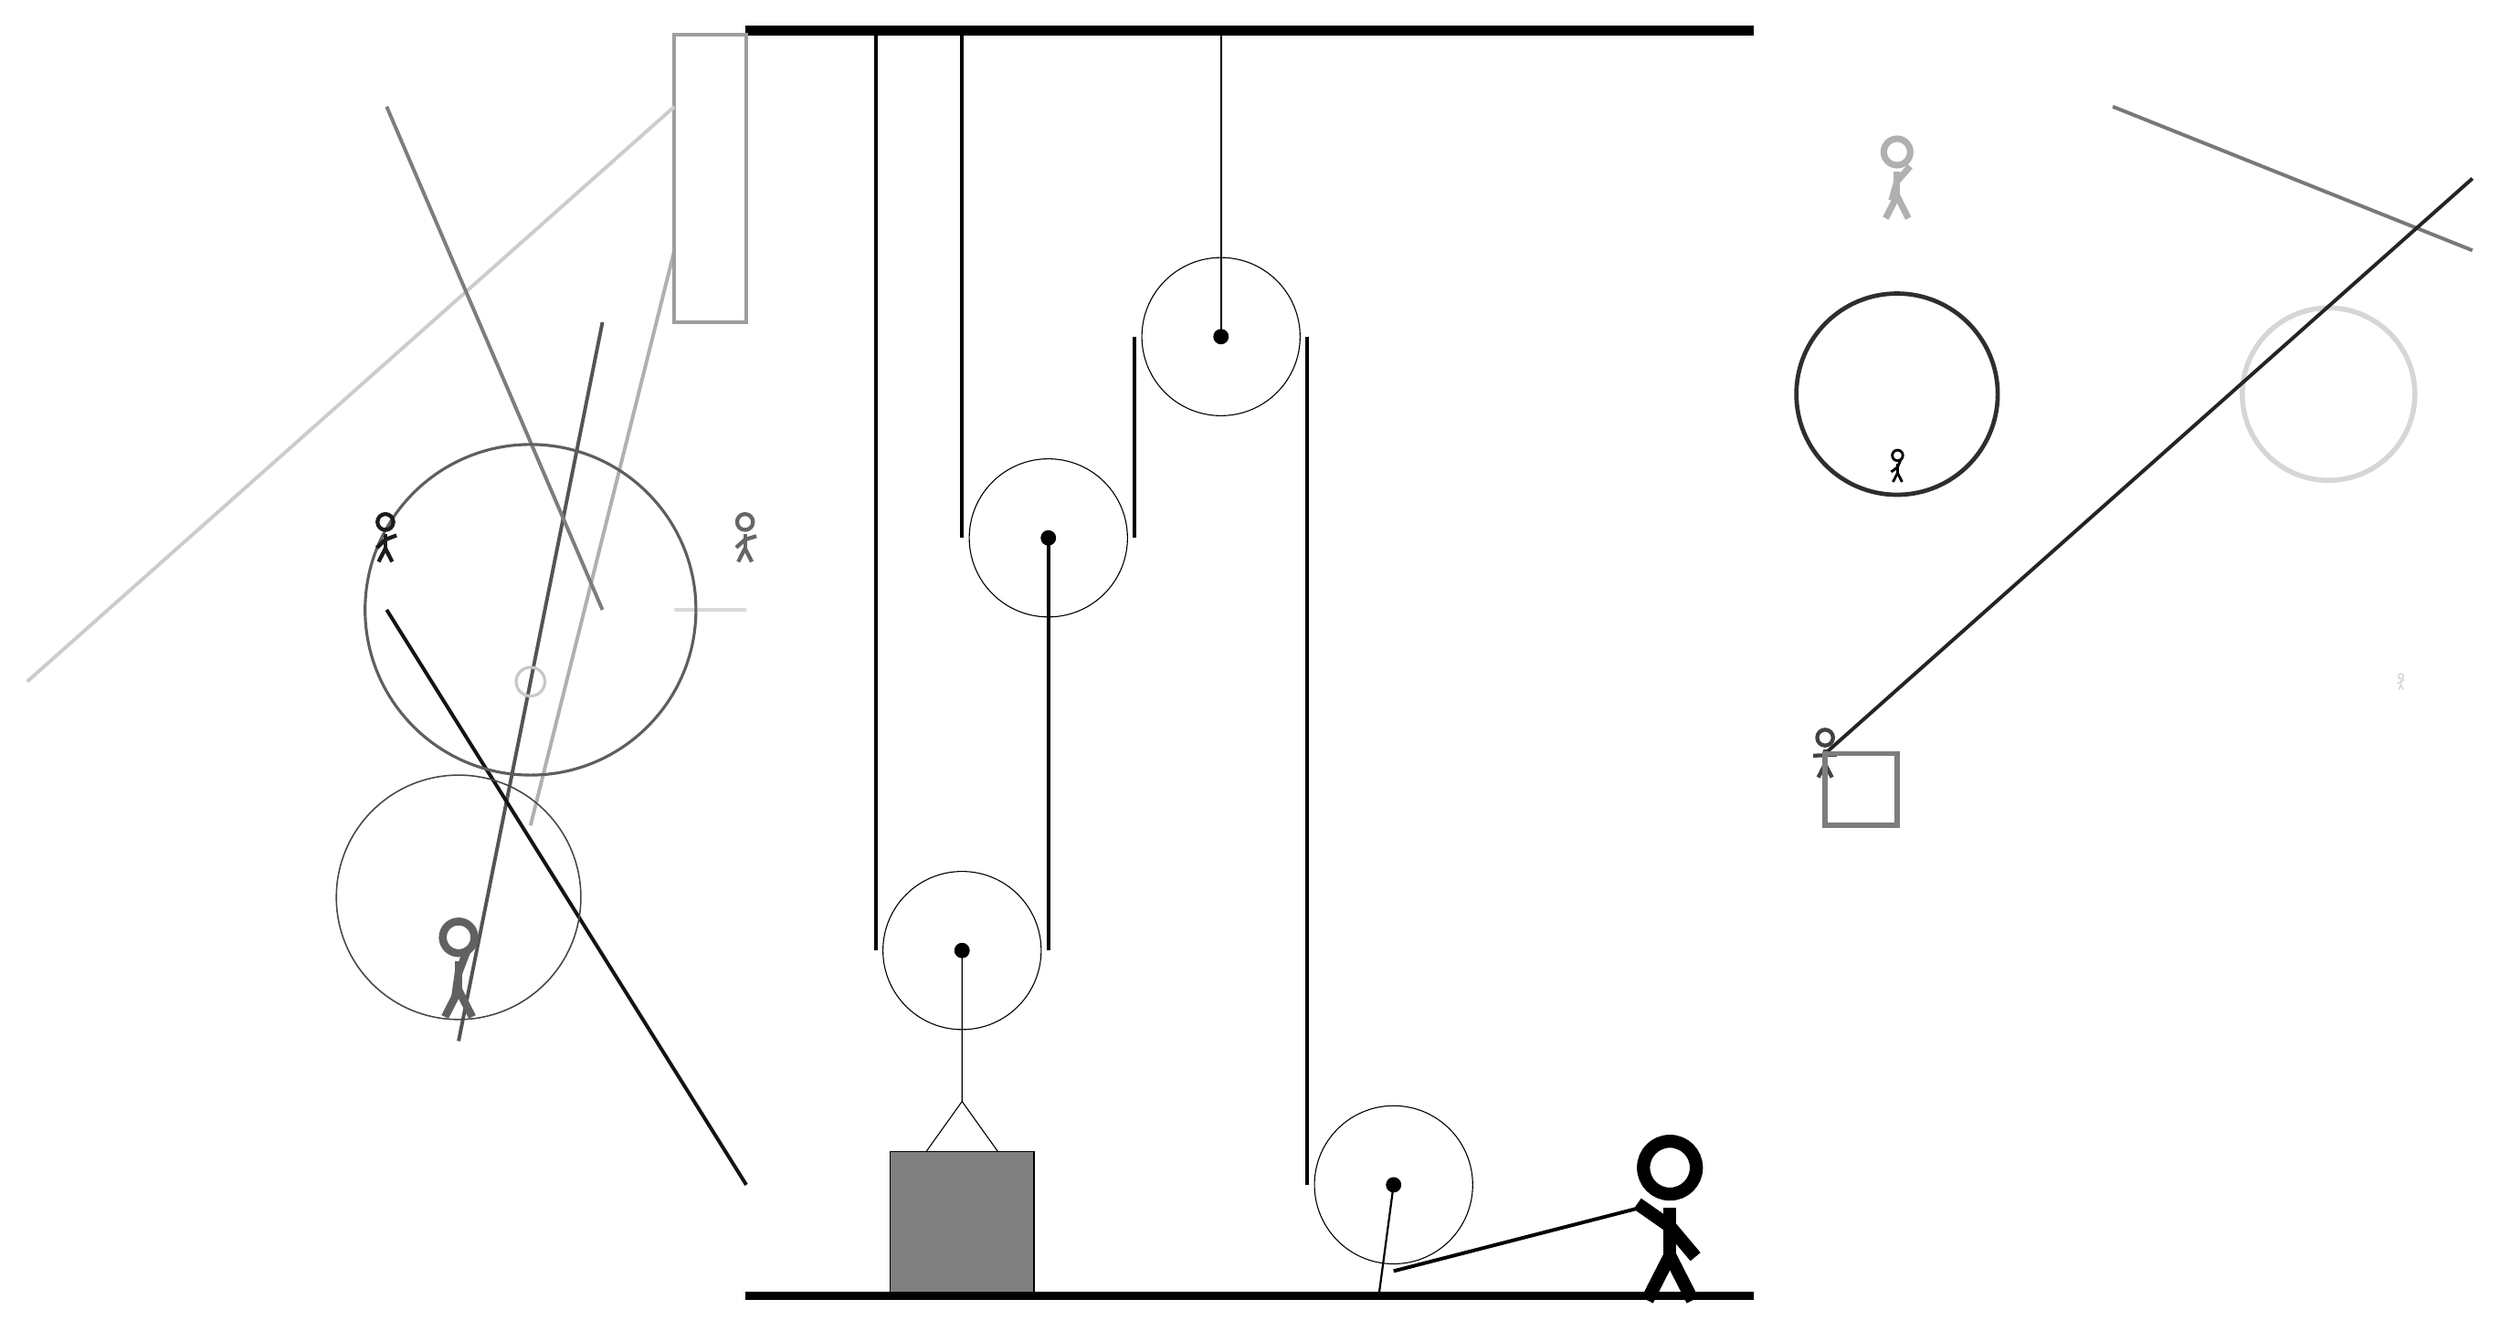
\begin{tikzpicture}
			%%%%% START %%%%%
			
			\draw[fill=black] (-2, 14) rectangle (12, 14.125);
			
			\draw (1, 1.26) circle (1.1);
			\draw[fill=black] (1, 1.26) circle (0.1);
			
			\draw (2.2, 7.0) circle (1.1);
			\draw[fill=black] (2.2, 7.0) circle (0.1);
			
			\draw (4.6, 9.8) circle (1.1);
			\draw[fill=black] (4.6, 9.8) circle (0.1);
			\draw[thick] (4.6, 9.8) -- (4.6, 14);
			
			\draw[line width=0.5mm, color=black!67](-4, 10) -- (-6, 0);
			
			\draw[line width=0.5mm, color=black!15] (-2, 6) rectangle (-3, 6);
			\draw [line width=0.7mm, color=black!16](20, 9) circle (1.2);
			\draw[line width=0.5mm, color=black!31](-3, 11) -- (-5, 3);
			\draw[line width=0.5mm, color=black!38] (-3, 14) rectangle (-2, 10);
			\draw[line width=0.5mm, color=black!53](17, 13) -- (22, 11);
			\node[line width=0.3mm, color=black!17] at (21, 5) {\Strichmaxerl[1][19][42]};
			\node[line width=0.5mm, color=black!60] at (-2, 7) {\Strichmaxerl[3][42][17]};
			\node[line width=0.6mm, color=black!31] at (14, 12) {\Strichmaxerl[5][74][49]};
			
			\draw[line width=0.5mm, color=black!20](-3, 13) -- (-12, 5);
			\draw[line width=0.5mm, color=black!86](13, 4) -- (22, 12);
			\draw[line width=0.5mm, color=black!51](-7, 13) -- (-4, 6);
			\draw[line width=0.5mm, color=black!92](-2, -2) -- (-7, 6);
			\draw [line width=0.6mm, color=black!82](14, 9) circle (1.4);
			\node[line width=0.4mm, color=black!74] at (13, 4) {\Strichmaxerl[3][2][0]};
			\draw [line width=0.4mm, color=black!22](-5, 5) circle (0.2);
			
			\draw [line width=0.4mm, color=black!63](-5, 6) circle (2.3);
			\draw[line width=0.7mm, color=black!51] (14, 4) rectangle (13, 3);
			\node[line width=0.4mm, color=black!89] at (-7, 7) {\Strichmaxerl[3][44][21]};
			
			\draw [line width=0.2mm, color=black!72](-6, 2) circle (1.7);
			\node[line width=0.6mm, color=black!100] at (14, 8) {\Strichmaxerl[2][37][67]};
			
			\node[line width=0.2mm, color=black!62] at (-6, 1) {\Strichmaxerl[6][82][69]};
			
			\draw (7.0, -2) circle (1.1);
			\draw[fill=black] (7.0, -2) circle (0.1);
			\draw[thick] (7.0, -2) -- (6.8, -3.5);
			
			\draw (1, 1.26) -- (1, -0.84) -- (0.5, -1.54) -- (1.5, -1.54) -- (1, -0.84);
			\draw[fill=black!50] (0, -1.54) rectangle (2, -3.54);
			\draw[line width=0.5mm] (-0.2, 14) -- (-0.2, 1.26);
			\centerarc[line width=0.5mm](1, 1.26)(180:360:1.2000000000000002);
			\draw[line width=0.5mm](2.2, 1.26) -- (2.2, 7.0);
			\draw[line width=0.5mm] (1.0, 14) -- (1.0, 7.0);
			\centerarc[line width=0.5mm](2.2, 7.0)(180:360:1.2000000000000002);
			\draw[line width=0.5mm](3.4, 7.0) -- (3.4, 9.8);
			\centerarc[line width=0.5mm](4.6, 9.8)(0:180:1.2000000000000002);
			\draw[line width=0.5mm] (5.8, 9.8) -- (5.8, -2);
			\centerarc[line width=0.5mm](7.0, -2)(0:90:-1.2000000000000002);
			\draw[line width=0.5mm](7.0, -3.2) -- (10.5, -2.3);
			
			\node at (10.8, -2.5) {\Strichmaxerl[10][-35][-50]};
			
			\draw[fill=black] (-2, -3.5) rectangle (12, -3.6);
			
			%%%%% END %%%%%
		\end{tikzpicture}
	\end{figure}	
\end{document}